\documentclass[tikz]{standalone}
\usepackage{tikz}
\usepackage{fourier}
\usepackage{physics}
\usetikzlibrary{shapes.geometric}
\usetikzlibrary{calc}

\begin{document}
\begin{tikzpicture}
    % Spherical harmonic plots
    \node[inner sep=0] at (0, 0) {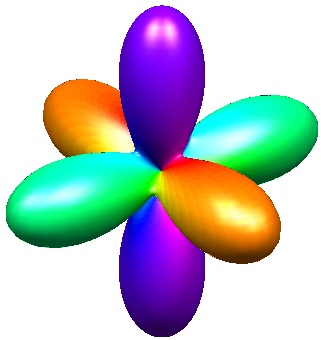
\includegraphics[scale=1.2]{../gfx/C1-spherical.pdf}};
    \node[inner sep=0] at (8, 0) {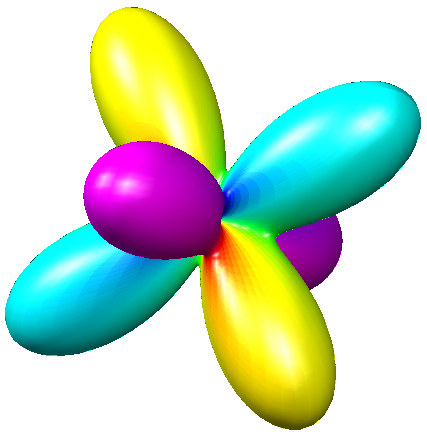
\includegraphics{../gfx/C2-spherical.pdf}};
    \node[inner sep=0] at (17, 0) {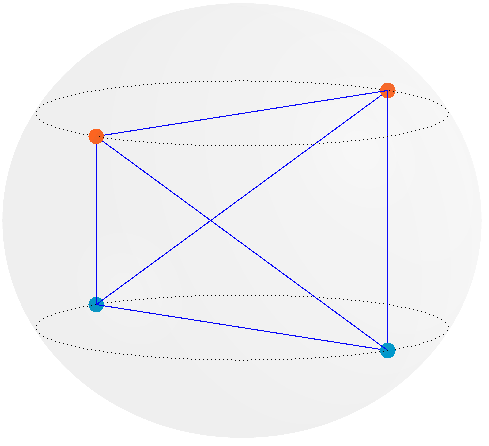
\includegraphics{../gfx/C1-Majorana.pdf}};
    \node[inner sep=0] at (26, 0) {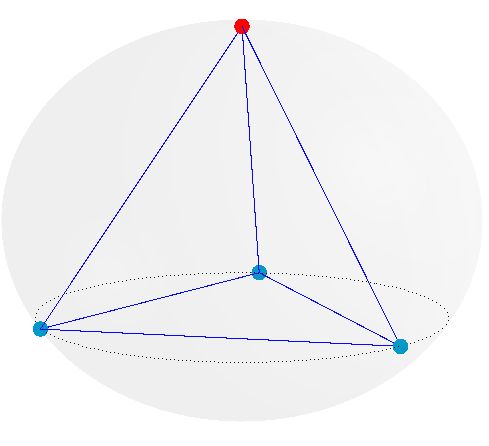
\includegraphics{../gfx/C2-Majorana.pdf}};

    % Colour bar
    \node[rotate=90] at (-4, 0) {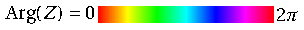
\includegraphics[scale=1.8]{../gfx/compiled_hsv.pdf}};
    \node at (31, 0) {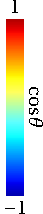
\includegraphics[scale=1.8]{../gfx/compiled_jet_majorana.pdf}};

    % Labels
    \node at (0, -5) {\Huge (a)};
    \node at (8, -5) {\Huge (b)};
    \node at (17, -5) {\Huge (c)};
    \node at (26, -5) {\Huge (d)};

    % C1 labels
    \draw[->, line width=2] (0, 3.3) -- (0, 4.1) node[above] {\Huge\(C_2\)};
    \draw[->, line width=2] (3.15, 1) -- (4, 1.5) node[above] {\Huge\(C_2\)};
    \draw[->, line width=2] (2.3, -1.6) -- (3.1, -2.) node[below] {\Huge\(C_2\)};
    \draw[->, line width=2] (0.3, 0.2) -- (2, 2) node[above] {\Huge\(C_3\)};

    % C2 labels
    \draw[->, line width=2] (8.2, 0) -- (8.2, 3) node[above] {\Huge\(C_3\)};
    \draw[->, line width=2] (11.3, 2) -- (12.1, 2.5) node[above] {\Huge\(C_2\)};
    \draw[->, line width=2] (6.3, 3.5) -- (5.9, 4.2) node[above] {\Huge\(C_2\)};
    \draw[->, line width=2] (10.1, -0.6) -- (10.6, -0.7) node[above] {\Huge\(C_2\)};

    % % BN Labels
    % \draw[->, line width=2] (7, 0) -- (7, 2) node[above] {\Huge \(C_4\)};
    % \draw[->, line width=2] (9.6, 2.2) -- (10.2, 2.8) node[above] {\Huge \(C_2\)};
    % \draw[->, line width=2] (8.4, 0.1) -- (10, 0.1) node[right] {\Huge \(C_2'\)};

    % Orientation
    \draw[->, line width=2] (-2.8, -4) -- (-2.8, -3) node[above] {\Huge \(z\)};
    \draw[->, line width=2] (-2.8, -4) -- (-1.8, -4) node[right] {\Huge \(x\)};
    \draw[->, line width=2] (-2.8, -4) -- (-2.2, -3.5) node[right] {\Huge \(y\)};

    % Spinor labels
    \node at (16, 4.4) {\huge \(\zeta^{\text{C}_1} = (1, 0, i\sqrt{2}, 0, 1)^T/2\)};
    \node at (25, 4.4) {\huge \(\zeta^{\text{C}_2} = (1, 0, 0, \sqrt{2}, 0)^T/\sqrt{3}\)};

\end{tikzpicture}
\end{document}

